\chapter{Neutron Scattering I}

\sourcepage{1}
\section{Objectives}
\begin{enumerate}
  \item Nuclear reactions and Bohr's independence hypothesis for the compound nucleus.
  \item The basic idea of a cross section as a way to describe reactions at the microscopic and macroscopic levels.
  \item The Schr\"odinger equation for two-body collisions and some special functions.
  \item A wave-mechanical description of scattering.
\end{enumerate}

\noindent Plus: administrivia.

\sourcepage{2}
\section{Review of relevant nuclear physics}
\textit{Mostly following B\&W.}

\subsection*{Course overview in brief}
The conceptual progression sketched in the notes is
\begin{center}
\begin{tikzpicture}[>=Latex,node distance=7mm and 7mm, every node/.style={align=center}]
  \node[draw,rounded corners] (sch) {Schr\"odinger equation};
  \node[draw,rounded corners,right=of sch] (nuc) {nuclear physics};
  \node[draw,rounded corners,right=of nuc] (rmat) {$R$-matrix and\\scattering ``laws''};
  \node[draw,rounded corners,below=of rmat] (xs) {cross sections};
  \node[draw,rounded corners,below=of xs] (modern) {modern neutron interactions};
  \node[draw,rounded corners,below left=8mm and -5mm of modern] (det) {deterministic\\continuum transport\\and various discretizations\\(Part II)};
  \node[draw,rounded corners,below right=8mm and -5mm of modern] (mc) {stochastic\\Monte Carlo\\(Part III)};
  \draw[->] (sch)--(nuc);
  \draw[->] (nuc)--(rmat);
  \draw[->] (rmat)--(xs);
  \draw[->] (xs)--(modern);
  \draw[->] (modern)--(mc);
  \draw[->] (modern)--(det);
\end{tikzpicture}
\end{center}
\marginnoteinline{Overlap with the Schr\"odinger-equation material builds off 22.101.  Experiments feed the $R$-matrix/scattering-law and cross-section descriptions.}

\subsection*{Some history}
\begin{description}[style=multiline,leftmargin=4em,labelwidth=3.2em]
  \item[1911] Rutherford discovers the nucleus, with positive charge $Z$.
  \item[1913] Thomson finds that charge $Z$ is not the mass; hence nuclei are not all protons.
  \item[1931] Ehrenfest and Oppenheimer note that a nucleus made from protons and electrons is inconsistent with angular momentum and statistics.  \marginnoteinline{Bose--Einstein versus Fermi statistics.}
  \item[1932] Chadwick and Curie--Joliot discover the neutron; Heisenberg suggests that nuclei are made of neutrons and protons.
\end{description}
Thus this is an approximately 80-year-old field: pretty young.

\sourcepage{3}
\section{Nuclear reactions and their classification}
Our interest is nuclear reactions,
\[
  a+X \longleftrightarrow Y+b,
\]
or, equivalently,
\[
  X(a,b)Y,
\]
or, when the context fixes the nuclei, simply $(a,b)$.

The notes classify reactions schematically as
\begin{center}
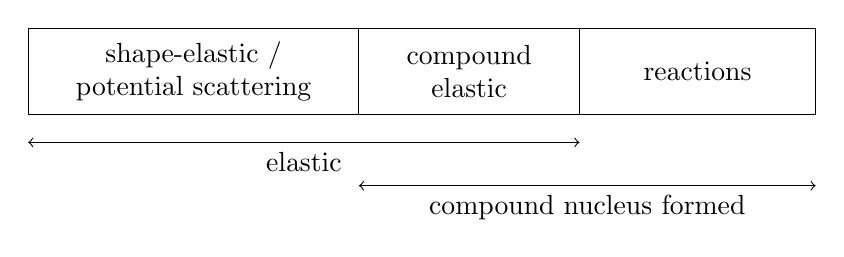
\begin{tikzpicture}[x=1cm,y=1cm]
  \draw (0,0) rectangle (10,1.1);
  \draw (4.2,0)--(4.2,1.1);
  \draw (7.0,0)--(7.0,1.1);
  \node[align=center] at (2.1,0.55) {shape-elastic /\\potential scattering};
  \node[align=center] at (5.6,0.55) {compound\\elastic};
  \node at (8.5,0.55) {reactions};
  \draw[<->] (0,-0.35)--node[below]{elastic}(7.0,-0.35);
  \draw[<->] (4.2,-0.9)--node[below]{compound nucleus formed}(10,-0.9);
\end{tikzpicture}
\end{center}
Elastic scattering conserves kinetic energy.  A reaction may involve energy loss, particle transfer, and so forth.  The objective is to quantify these processes in terms of their probability of occurring.

\sourcepage{4}
\section{Reaction cross section}
A generic reaction cross section is written as
\[
  \sigma
  =\frac{\text{number of events of a certain type per unit time}}
  {\text{number of incident particles per unit area per unit time}}.
\]

Typical reaction forms are
\[
  a+x \longrightarrow
  \begin{cases}
    x+a, & \text{elastic},\\
    x^*+a, & \text{inelastic},\\
    Y+b,\\
    Z+c,
  \end{cases}
\]
where the last two lines represent other processes, such as radiative capture, fission, or an $(n,\alpha)$ reaction.

For example, in $a+x\to x^*+a$, the nucleus $X$ may have many possible excited states, $X^*,X^\dagger,X',\ldots$.  Any outcome $X^{\beta'}+a^{\beta''}$ satisfying the conservation laws is a \emph{reaction channel}.  The entrance and exit channels are distinguished.  The quantities $\alpha$ and $\beta$ describe the quantum states of the entrance and exit systems.

A reaction outcome must conserve
\begin{enumerate}
  \item number of nucleons,
  \item charge,
  \item mass--energy,
  \item linear and angular momentum,
  \item parity.
\end{enumerate}

\sourcepage{5}
We want to quantify these reactions with respect to their probability of occurring.  The generic definition is
\[
  \sigma
  =\frac{\text{number of events of a certain type per unit time and area}}
  {\text{number of incident particles per unit time and area}}.
\]
The dimensions are those of area,
\[
  [\sigma]=\unit{cm^2},
  \qquad
  1\unit{b}=10^{-24}\unit{cm^2},
\]
where $\mathrm{b}$ denotes a barn.

\subsection*{Application to a slab}
Consider a slab in which $\sigma$ represents one type of reaction (or all reactions together).  Let $I_0$ be the incident intensity, with units of particles per square centimeter per second; let $I(x)$ be the intensity at depth $x$; and let $N$ be the target number density in targets per cubic centimeter.  Over a thickness $\dd x$, the number of targets per unit area is $N\dd x$.  The number of collisions per unit time and unit area is proportional to $I$ and $N\dd x$, with proportionality constant $\sigma$.  Thus
\[
  \dd I=-\sigma I N\dd x.
\]

\sourcepage{6}
Integration gives
\[
  I(x)=I_0\ee^{-N\sigma x}.
\]
The units are consistent because
\[
  [N][\sigma]=[\unit{cm^{-3}}][\unit{cm^2}]=[\unit{cm^{-1}}].
\]
Define the macroscopic cross section
\[
  \Sigma=N\sigma,
\]
with, for a material mixture,
\[
  N=\frac{N_A\rho}{M}.
\]
The symbol $\sigma$ is then the microscopic cross section, and $\Sigma^{-1}$ is the mean free path.

Taking $I_0=1$, the probability that a particle reaches $x$ without colliding is
\[
  P(\text{reaches }x)=\ee^{-\Sigma x}.
\]
The probability that it first collides in $[x,x+\dd x]$ is
\[
  P(\text{reaches }x\text{ and then collides})
  =\left|\frac{\dd I}{\dd x}\right|_{x}\dd x\,\ee^{-\Sigma x}
  =\Sigma\ee^{-\Sigma x}\dd x.
\]
The mean distance to collision is therefore
\[
  \overline{x}
  =\frac{\int_0^\infty x\Sigma\ee^{-\Sigma x}\dd x}
  {\int_0^\infty \Sigma\ee^{-\Sigma x}\dd x}
  =\frac{1}{\Sigma}.
\]
\marginnoteinline{Exercise in the notes: carry out the mean-free-path integral.}

\sourcepage{7}
All reactions except potential scattering proceed through formation of a compound nucleus, and such reactions are much more probable at discrete energies: resonances.

\section{Bohr's independence hypothesis}
A compound-nucleus reaction is a two-stage process:
\begin{enumerate}
  \item Formation of a compound system:
  \[
    C:\quad a+X\longrightarrow C.
  \]
  \item Decay of $C$ into reaction products:
  \[
    C\longrightarrow Y+b.
  \]
\end{enumerate}
The key idea is that stages 1 and 2 are independent.

Why is this plausible?  The incident neutron quickly shares its energy within the nucleus.  The notes estimate a neutron mean free path within a nucleus of order $10^{-14}\unit{cm}$, whereas the nuclear radius is approximately
\[
  R\sim 1.2A^{1/3}10^{-13}\unit{cm}.
\]
Taking a nucleon cross section of order one barn,
\[
  \Sigma_{\text{nucleon}}\sim \rho\sigma.
\]

\sourcepage{8}
The rough density estimate in the notes is
\begin{align*}
  \Sigma_{\text{nucleon}}
  &\sim \rho\sigma\\
  &\sim \frac{A}{\frac{4}{3}\pi\left[1.2A^{1/3}10^{-13}\right]^3}\,\sigma\\
  &\sim \frac{3}{1.8\,4\pi\,10^{-39}}10^{-24}\\
  &\sim 10^{14}\unit{cm^{-1}}.
\end{align*}
The following handwritten line reads
\[
  \text{MFP}\sim 10^{-19}\unit{cm}.
\]
% TRANSCRIPTION NOTE: the source clearly appears to say 10^{-19} cm, although the immediately preceding estimate would imply 10^{-14} cm and source page 7 states 10^{-14} cm.

It takes a relatively long time for the energy to concentrate in one particle for subsequent ejection.  This happens through multiple exchanges.  As long as the average excitation energy per nucleon is well below the separation energy, many exchanges are expected before decay.  This is why the compound nucleus does not ``remember'' how it got there: the long time causes it to ``forget'' how it formed.

An alternative uncertainty-principle argument is sketched: if the resonance width is of order electron-volts, then
\[
  \Delta E\,\Delta t\sim\hbar
  \quad\Longrightarrow\quad
  \Delta t\sim 10^{-16}\unit{s}
\]
for a representative $\Delta E\sim 100\unit{eV}$.  Compared with a crossing time of roughly $10^{-19}\unit{s}$, the compound nucleus exists for many crossing times and therefore loses memory of the entrance process.

\sourcepage{9}
Define $\alpha$ as the incident channel and $\beta$ as an exit channel.  Generalizing the cross section,
\[
  \sigma_{\alpha\beta}
  =\frac{\text{number of emissions into channel $\beta$ per unit time per scattering center}}
  {\text{number of incident particles in channel $\alpha$ per unit area per unit time}}.
\]
With Bohr's hypothesis,
\[
  \sigma_{\alpha\beta}=\sigma_{\alpha C}G_{C\beta},
\]
where $\sigma_{\alpha C}$ is the cross section for formation of the compound nucleus and $G_{C\beta}$ is the probability that, once formed, $C$ decays into channel $\beta$.  This is the branching ratio, with
\[
  \sum_{\beta}G_{C\beta}=1.
\]

\sourcepage{10}
Use
\[
  \hbar=6.582\times 10^{-22}\unit{MeV\,s}.
\]
\marginnoteinline{Leave total and partial widths, level widths, and level spacings for the continuum treatment.}

For a compound nucleus $C$ at excitation energy $E_C$, define the mean lifetime
\[
  \tau_C(E_C)=\text{mean lifetime of compound nucleus $C$ with energy $E_C$}.
\]
The total width is
\[
  \Gamma(E_C)=\frac{\hbar}{\tau_C},
\]
which has units of energy and is analogous to a decay rate.  A partial width $\Gamma_\beta(E_C)$ satisfies
\[
  \sum_{\beta\ \text{open}}\Gamma_\beta=\Gamma.
\]
Hence
\[
  G_{C\beta}(E_C)=\frac{\Gamma_\beta(E_C)}{\Gamma(E_C)}.
\]
The notes also record
\[
  \Gamma\tau=\hbar
\]
and the uncertainty relation
\[
  \Delta E\,\Delta t\sim\hbar.
\]
Because the lifetime $\tau$ is finite, $\Delta E$ is nonzero; therefore resonances are not delta functions in energy.
